\documentclass[12pt,a4paper,titlepage]{report}
\usepackage{graphicx}
\usepackage[left=2.8cm, right=2.2cm, top=3cm, bottom=2.5cm]{geometry}
\usepackage{latexsym}		% to get LASY symbols
\usepackage{epsfig}			% to insert PostScript figures
\usepackage{eufrak}
\usepackage{type1cm}
\usepackage{newsec}
\usepackage{titlesec}
\usepackage{longtable}
\usepackage{url}
\usepackage[export]{adjustbox}
\usepackage{listings}
\usepackage{xcolor}
\usepackage{pdfpages}
\usepackage{caption}
\usepackage{listings}
\usepackage{float}
\usepackage{acro}

\definecolor{customgreen}{rgb}{0,0.6,0}
\definecolor{customgray}{rgb}{0.5,0.5,0.5}
\definecolor{custommauve}{rgb}{0.6,0,0.8}
\lstdefinelanguage{HTML}{
	sensitive=true,
	keywords={},
	otherkeywords={<, >, /},
	morecomment=[s]{<!--}{-->},
	morestring=[b]"
}


\lstset{ 
	basicstyle=\small,        % the size of the fonts that are used for the code
	breaklines=true,                 % sets automatic line breaking
	commentstyle=\color{customgreen},    % comment style
	firstnumber=1,                % start line enumeration with line 1000
	frame=single,	                   % adds a frame around the code
	keepspaces=true,                 % keeps spaces in text, useful for keeping indentation of code (possibly needs columns=flexible)
	keywordstyle=\color{blue},       % keyword style
	numbers=left,                    % where to put the line-numbers; possible values are (none, left, right)
	numbersep=10pt,                   % how far the line-numbers are from the code
	numberstyle=\tiny\color{customgray}, % the style that is used for the line-numbers
	rulecolor=\color{black},         % if not set, the frame-color may be changed on line-breaks within not-black text (e.g. comments (green here))
	showspaces=false,                % show spaces everywhere adding particular underscores; it overrides 'showstringspaces'
	showstringspaces=false,          % underline spaces within strings only
	showtabs=false,                  % show tabs within strings adding particular underscores
	stepnumber=1,                    % the step between two line-numbers. If it's 1, each line will be numbered
	stringstyle=\color{custommauve},     % string literal style
	tabsize=2,	                   % sets default tabsize to 2 spaces
	title=\lstname                   % show the filename of files included with \lstinputlisting; also try caption instead of title
}


\titleformat{\chapter}[display]
{\normalfont\Large\bfseries\centering}{\chaptertitlename\
	\thechapter}{25pt}{\Large}
\titleformat{\section}{\normalfont\bfseries}{\noindent\thesection}{20pt}{}
\titleformat{\subsection}{\normalfont\small\bfseries}{\thesubsection}{15pt}{\small}
\titlespacing*{\chapter}{0pt}{0pt}{40pt}


\begin{document}
	\titlepage
	\thispagestyle{empty}
	\begin{center}
		
\includegraphics[scale=0.3]{logo1.png}\\[0.5cm]
		\large \textit{Mini Project Report On}\\[0.6cm]
		\Large \textbf{Malayalam Parser for Dataset Creation }\\[0.6cm]
		\textit{Submitted in partial fulfillment of the
			requirements for the award of the degree of}\\[0.6cm]
		{\huge {$\mathfrak {Bachelor\; of\; Technology}$}}\\[.2cm]
		%{\Large {$\mathfrak {In}$}}\\[.5cm]
		%{\Large {$\mathfrak {Computer\; Science\; \&\; Engineering}$}}\\[2cm]
		\textit{in}\\[.2cm]
		{\Large \bf \itshape{{Computer\; Science\; \&\; Engineering}}}\\[0.4cm]
		\large \bfseries{By}\\[.4cm]
		\large \bfseries{ Fathima Jennath N.K (U2103089) }\\[0.2cm]
		\large \bfseries{ Gautham C Sudheer (U2103092) }\\[0.2cm]
		\large \bfseries{ Godwin Gino (U2103096) }\\[0.2cm]
		\large \bfseries{ Mohammed Basil (U2103139) }\\[0.6cm]
		\large \bfseries{Under the guidance of}\\[0.75cm]
		\large \bfseries{Dr.Mary Priya Sebastian}\\[0.75cm]
		%		
\includegraphics[width=8.0cm]{logo (1).jpg}\\[0.5cm]
		\large \textbf{Department of Computer\; Science\; \&\; Engineering}\\
		\large \textbf{Rajagiri School of Engineering \&\ Technology (Autonomous)}\\
		\small \bfseries{(Affiliated to APJ Abdul Kalam Technological University)}\\
		\large \textbf{Rajagiri Valley, Kakkanad, Kochi, 682039}\\
		\large \bfseries{May 2024}
	\end{center}
	
	\newpage
	\thispagestyle{empty}
	\begin{center}
		%	\textbf {DEPARTMENT OF COMPUTER SCIENCE \&\ ENGINEERING}\\
		%	\small \textbf{RAJAGIRI SCHOOL OF ENGINEERING \&\ TECHNOLOGY (AUTONOMOUS)}\\
		
		%	\small \textbf{RAJAGIRI VALLEY, KAKKANAD, KOCHI, 682039}\\
		%   \small \bfseries{(Affiliated to APJ Abdul Kalam Technological University)}\\[0.5cm]
		%\begin{figure}[htbp]
		%	\centering
		%
\includegraphics[scale=0.40]{logo (1).jpg}
		%   
\includegraphics[width=8.0cm]{logo (1).jpg}\\[0.5cm]
		%\end{figure}
		\large \bfseries{\huge{CERTIFICATE}}\\[5cm]
	\end{center}
	
	\renewcommand{\baselinestretch}{1.2}\normalsize
	
	\emph{This is to certify that the mini project report entitled \textbf{"Malayalam Parser for Dataset Creation”} is a bonafide record of the work done by \textbf{Fathima Jennath N.K (U2103089)}, \textbf{Gautham C Sudheer (U2103092)}, \textbf{Godwin Gino (U2103096)}, \textbf{Mohammed Basil (U2103139)}, submitted to the APJ Abdul Kalam Technological University in 
		partial fulfillment of the requirements for the award of the degree of Bachelor of Technology (B. Tech.) in Computer Science and Engineering during the academic year 2023-2024.}\\[2.5cm]
	
	\begin{flushleft}
		
		
		\begin{longtable}{p{10.3cm} p{8cm} p{5.25cm}}
			%	\small\textbf{Name of Guide}    &\small\textbf{Name of Coordinator} \\
			{Dr.Mary Priya Sebastian}& {Dr.Saritha S}\\
			{Associate Professor}& {Professor}\\
			{Dept. of CSE}&  {Dept. of CSE}\\
			{RSET} ~&{RSET} \\
			
		\end{longtable}
	\end{flushleft}
	
	\begin{center}
		%\small\textbf{Name of HoD}\\
		{Dr.Preetha K.G}\\
		{Head of the Department}\\
		{Dept. of CSE}\\
		{RSET}
	\end{center}	
	
	
	
	
	
	
	\renewcommand{\baselinestretch}{1.5}\normalsize
	\newpage
	%\renewcommand\abstractname{ACKNOWLEDGEMENTS}
	\chapter*{ACKNOWLEDGEMENTS}
	%\begin{abstract}
	\pagenumbering{roman}
	\setcounter{page}{1}
	\addcontentsline{toc}{chapter}{Acknowledgements}
	\vspace{1.5cm}
	%\begin{spacing}{}
	\paragraph\ I wish to express my sincere gratitude towards Dr P. S. Sreejith, Principal of RSET, and Dr. Preetha K.G., Head of the Department of Computer Science and Engineering for providing me with the opportunity to undertake my mini project, "Malayalam Parser for Dataset Creation".
	\paragraph\ I am highly indebted to my project coordinator, \textbf{Dr.Saritha S}, Professor, Department of Computer Science and Engineering for their valuable support.
	
	\paragraph\ It is indeed my pleasure and a moment of satisfaction for me to express my sincere
	gratitude to my project guide \textbf{Dr.Mary Priya Sebastian} for her patience and all the priceless advice and  wisdom she has shared with me.
	\paragraph\ Last but not the least, I would like to express my sincere gratitude towards all other teachers and friends for their continuous support and constructive ideas.
	
	%\end{spacing}
	\begin{flushright}
		\textbf{Fathima Jennath NK}\\
		\textbf{Gautham C Sudheer}\\
		\textbf{Godwin Gino}\\
		\textbf{Mohammed Basil}
	\end{flushright}
	
	
	%\end{abstract}
	
	
	\newpage
	
	\renewcommand{\baselinestretch}{1.5}\normalsize
	%\thispagestyle{empty}
	%\renewcommand\abstractname{ABSTRACT}
	
	\chapter*{Abstract}
	%\begin{abstract}
	%	\pagenumbering{roman}
	%	\setcounter{page}{3}
	\addcontentsline{toc}{chapter}{Abstract}
	\vspace{1.5cm}
	\paragraph\ \ \ \ The “Malayalam Parser for Dataset Creation” project aims to address the scarcity of annotated datasets in the Malayalam language for Natural Language Processing (NLP) applications. The primary objective is to develop a robust Malayalam parser capable of analyzing the syntactic and
	semantic structures of Malayalam sentences. The creation of this parser involves several key steps, including data collection from diverse sources, preprocessing to ensure data quality, and man-ual annotation of a representative subset of the data with grammatical and syntactic information.
	The parser development process encompasses the selection of an appropriate parsing approach,whether rule-based, statistical, or machine learning-based. The model is trained using the annotated Malayalam dataset, focusing on capturing the unique linguistic nuances of the Malayalam language. Evaluation metrics are employed to assess the parser’s performance on a separate test
	set, guiding iterative refinement and enhancement. The resulting Malayalam parser serves as a valuable tool for the analysis of grammatical structures in new Malayalam text data. Its application contributes to the creation of high-quality Malayalam datasets, crucial for advancing NLP research
	and applications in the Malayalam language. This project encourages collaboration with linguists,researchers, and the Malayalam-speaking community to ensure linguistic accuracy and relevance in the development of the parser. The “Malayalam Parser for Dataset Creation” project aligns with the broader goal of promoting linguistic diversity in NLP, addressing the challenges posed by the scarcity of resources for underrepresented languages. Through the development of this parser, the project aims to facilitate further research and innovation in Malayalam NLP, opening avenues for the exploration of various language-related tasks and applications.
	
	%\end{spacing}
	%\end{abstract}
	
	
	\newpage
	\normalsize{}
	
	%\pagenumbering{roman}
	%\setcounter{page}{4}
	%\begin{spacing}{}
	\tableofcontents
	%\end{spacing}
	% \thispagestyle{empty}
	\newpage
	
	
	\listoffigures
	\addcontentsline{toc}{chapter}{List of Figures}
	% \thispagestyle{empty}
	\newpage
	
	
	% \pagenumbering{roman}
	%\setcounter{page}{9}
	\listoftables
	\addcontentsline{toc}{chapter}{List of Tables}
	%	\addcontentsline{toc}{chapter}{List of Abbreviations}
	%	\listof{Abbreviations}
	% \thispagestyle{empty}
	\newpage
	
	\chapter*{List of Abbreviations}
	\addcontentsline{toc}{chapter}{List of Abbreviations}
	
		 NLP - Natural Language Processing
		 \newline
		 NER - Named Entity Recognition
		 \newline
		 POS - Part-of-Speech
	
	
	
	
	\newpage
	
	\cleardoublepage
	
	\pagenumbering{arabic}
	\setcounter{page}{1}
	%\begin{spacing}{}
	\chapter{Introduction}
	
	\section{Background}
	
	Malayalam is spoken widely in Kerala and neighboring areas but has not received as much attention in the tech world as bigger languages like English. This lack of attention has led to a scarcity of tools for analyzing Malayalam text, despite its complex grammar and word forms.
	\newline
	Our project aims to address this issue by creating a specialized system for Malayalam that can understand and process Malayalam text more effectively than current tools. This system will facilitate tasks such as sentiment analysis, translation, and summarization, benefiting areas such as education and business.
	\newline
	We are designing our system to be adaptable and scalable, ensuring that it can evolve to meet diverse needs. Our ultimate goal is to establish a strong foundation for Malayalam language technology, paving the way for future improvements and innovations.
	\newline
	In short, our project focuses on using technology to make working with Malayalam text more efficient, enabling individuals to achieve more in various fields.
	
	
	
	
	
	\section{Problem Definition}
	
	The aim of the project is to create a Malayalam Parser for Dataset Creation, involving data collection, preprocessing, manual annotation, and training using various parsing approaches to address the scarcity of annotated datasets in Malayalam for NLP applications.
	
	
	\section{Scope and Motivation}
	
	\textbf{Scope:}
	\newline
	The Malayalam Parser project aims to develop an advanced tool capable of
	understanding and processing Malayalam text efficiently. It encompasses essential
	tasks such as tokenization, part-of-speech tagging, parsing, and semantic analysis,
	providing a comprehensive breakdown of Malayalam sentences. The system's scope
	extends to facilitating tasks such as identifying different parts of speech and
	extracting meaningful insights from text. Additionally, the parser's design includes
	provisions for future expansion, allowing for the incorporation of domain-specific or specialized parsing tasks. This flexibility ensures that the parser can adapt to
	evolving needs and requirements, making it applicable across various domains and
	applications.
	\newline
	\textbf{Motivation:}
	\newline
	The motivation behind the Malayalam Parser project stems from the necessity for effective tools to process Malayalam text, essential for informed decision-making and strategic planning. By implementing parsing tasks such as tokenization, part-of-
	speech tagging, parsing, and semantic analysis, the system enables data-driven decision-making processes, enhancing strategic planning and execution.Furthermore, the project's innovation lies in the creation of annotated datasets,crucial for training and evaluating models for sentiment analysis, machine translation,question answering, and domain-specific parsing. Through these efforts, the project aims to advance natural language processing capabilities in Malayalam, contributing to the improvement of Malayalam language processing technologies and fostering innovation in linguistic research and technology development.
	
	
	
	
	\begin{center}
		\begin{tabular}{|c|p{12cm}|}
			\hline
			\textbf{Parsing Tasks} & \textbf{Description} \\
			\hline
			Tokenization & Breaking down sentences into individual words or tokens. \\
			\hline
			Part-of-Speech Tagging & Assigning grammatical tags to each word in a sentence. \\
			\hline
			Parsing & Analyzing the structure of sentences to understand their grammatical relationships. \\
			\hline
			Semantic Analysis & Extracting the meaning and context from sentences. \\
			\hline
		\end{tabular}
		\captionof{table}{Description of parsing tasks}
		\label{tab:parsing_tasks}
	\end{center}
	
	
	\section{Objectives}
	
	\begin{itemize}
		\item Develop parsing algorithms to accurately identify linguistic
		components such as words, phrases, and sentences in Malayalam
		text, laying the foundation for comprehensive analysis.
		\item Implement functionalities to determine the grammatical structure,
		syntax, and semantics of Malayalam sentences, facilitating precise
		linguistic analysis and comprehension.
		\item Incorporate part-of-speech tagging, syntactic parsing, and
		semantic analysis capabilities tailored specifically for the
		Malayalam language, enabling detailed linguistic processing.
		\item Enhance the Malayalam Parser system to effectively handle
		compound words, inflections, and variations in word forms
		commonly encountered in Malayalam text, ensuring robust parsing
		capabilities.
		\item Ensure compatibility and interoperability with existing linguistic
		analysis frameworks, facilitating seamless integration and
		utilization of the Malayalam Parser within broader NLP
		applications.
		\item Continuously refine and optimize the Malayalam Parser system to
		improve efficiency, accuracy, and adaptability in analyzing and
		processing Malayalam text data.
	\end{itemize}
	
	\section{Challenges}
	\begin{enumerate}
		\item Morphological Complexity: Malayalam words can change a lot by adding suffixes, making it hard for the parser to figure out their basic forms and parts of speech. This makes it tough to understand the meaning and grammar of sentences.
		\item Limited Resources: The scarcity of Malayalam-specific NLP tools and datasets complicates the development and training process. Adapting existing tools from other languages or creating new ones becomes necessary, potentially slowing down progress and hindering the effectiveness of the parser.
		\item Syntactic Freedom: Malayalam's relatively flexible sentence structure allows for varied word orders, challenging parsing algorithms in determining precise word relationships. This freedom introduces complexity in identifying grammatical elements like subjects, objects, and verbs, especially when word order isn't a definitive indicator.
		\item Data Annotation: The process of manually annotating data for parts of speech (POS), named entities, and intents is meticulous and time-consuming, requiring expertise in Malayalam grammar. It's crucial to ensure the quality and comprehensiveness of annotated training data for the parser's success, although this can be resource-intensive.
		\item Model Selection and Training: Optimal performance of POS tagging, named entity recognition, and intent recognition tasks relies on choosing suitable algorithms and training them effectively. However, training on potentially limited or imbalanced datasets necessitates careful optimization, such as data augmentation and hyperparameter tuning, to mitigate any shortcomings. 
	\end{enumerate}
	
	
	
	
	\section{Assumptions}
	
	\begin{enumerate}
		\item Availability of Training Data: The project assumes a certain amount of high-quality Malayalam text data will be available for annotation and training the parser for POS tagging, NER, and intent recognition.
		\item Effectiveness of Algorithms: The project assumes that the selected algorithms for POS tagging, NER, and intent recognition will be capable of accurately handling the linguistic complexities inherent in the Malayalam language.
		\item Computational Resources: Adequate computational resources are assumed to be accessible for training the parser models, as this process can be computationally demanding.
		\item Annotation Quality: The project assumes the quality of the annotations in the training data, including accuracy and consistency, as these factors greatly influence the performance of the parser models.
		
	\end{enumerate}
	
	
	\section{Societal / Industrial Relevance}
	
	The project aims to preserve and promote Malayalam, enhancing understanding and analysis of Malayalam text, providing datasets for parts-of-speech tagging, named entity recognition, and intent recognition. It supports research and learning in NLP and Malayalam linguistics, improving access to information for Malayalam speakers online. The project also supports the development of local language technologies for industries in Malayalam-speaking regions, expanding market opportunities in e-commerce and social media.
	
	
	\section{Organization of the Report}
	
	The organization of the report are as follows:
	\begin{itemize}
		\item 	\textbf{Chapter 1-Introduction:}The introduction covers the background of the project, the problem definition, the scope and motivation, the objectives,the societal and industrial relevance, the assumptions and the challenges faced by the project.
		
		\item \textbf{Chapter 2-Software Requirements Specification:} This chapter outlines the functional and nonfunctional requirements of the NLP tools for Malayalam. It defines the overall description of the software, external interface requirements, system features, and other nonfunctional requirements necessary for the development and deployment of the tools.
		
		\item \textbf{Chapter 3-System Architecture and Design:} The system architecture and design chapter provides an overview of the project’s technical framework. It includes discussions on the system overview, architectural design, identified datasets, proposed algorithms, implementation strategies, module division, and a work schedule presented as a Gantt chart for project planning and management.
	\end{itemize}
	
	
	
	
	
	
	
	\chapter{Software Requirements Specification}
	
	
	\section{Introduction}
	\subsection{Purpose}
	\paragraph\
	The system aims to enhance the understanding and analysis of Malayalam text data, enabling more
	accurate and efficient processing of information, including but not limited to retrieval, sentiment
	analysis, machine translation, and text summarization. By focusing on the unique linguistic characteristics
	of Malayalam, the project seeks to overcome the challenges posed by the language’s morphology,
	syntax, and semantics. Through the development of innovative algorithms, data structures, and
	linguistic resources, the project aims to contribute to the advancement of NLP research and technology
	in the context of the Malayalam language.
	\begin{itemize}
		\item 	 The primary focus of the Malayalam Parser system is to analyze and parse written text in
		the Malayalam language. This involves tasks such as tokenization, part-of-speech tagging,
		parsing, and semantic analysis.
		\item Initially, the system will target general-purpose parsing tasks, which are applicable to a wide
		range of text data. These tasks form the foundation of the parsing capabilities of the system.
		\item The system is designed to be extensible, allowing for the inclusion of domain-specific or
		specialized parsing tasks in the future. This flexibility ensures that the system can adapt to
		different needs and requirements over time.
		\item In addition to algorithms and data structures, the project also involves the development of
		linguistic resources that are crucial for parsing Malayalam text. These resources may include
		lexicons, grammars, and annotated corpora.
	\end{itemize}
		
	
    \subsection{Product Scope}
    \paragraph\
    The Malayalam Parser is a smart tool that understands Malayalam text. It breaks down sentences to
    figure out their grammar, structure, and meaning using advanced language processing techniques.
    It helps with tasks like identifying different parts of speech, understanding how sentences are put
    together, and analyzing the overall meaning of text.
    \begin{enumerate}
    	
    	\item \textbf{Informed Decision-Making:} Implementation of parsing tasks including tokenization, part-of-speech tagging, parsing, and semantic analysis for Malayalam text. Extracting insights from Malayalam text aids in data-driven decision-making, enhancing strategic planning and
    	execution.
    	\item \textbf{Innovation:} Developing a Malayalam parser for dataset creation is significant as it encompasses
    	crucial linguistic tasks such as tokenization, part-of-speech tagging, and named entity recognition.
    	This effort is essential for advancing natural language processing capabilities in Malayalam,
    	enabling the development of robust models for sentiment analysis, machine translation,
    	question answering, and domain-specific parsing. The creation of annotated datasets is vital
    	to train and evaluate these models, contributing to the overall improvement of Malayalam
    	language processing technologies.
    \end{enumerate}
	
	
	\section{Overall Description}
	\subsection{Product Perspective}
	\paragraph\
	This software represents a new, standalone product developed to fulfill the crucial task of parsing
	and analyzing Malayalam language text. Unlike existing systems or components, this software
	is designed from the ground up to specialize in the intricacies of Malayalam language parsing,
	catering to the specific needs of users requiring accurate linguistic analysis in Malayalam.
	The Malayalam Parser software does not belong to a product family but serves as an independent
	solution, tailored specifically for parsing Malayalam text. It is not intended as a replacement for
	existing systems but rather as a complementary tool to enhance language processing capabilities in
	Malayalam. While it operates autonomously, it may interface with other systems or applications,
	such as text input sources or linguistic databases, to facilitate seamless integration within broader
	linguistic analysis frameworks.
	\begin{figure}[H]
		\centering
		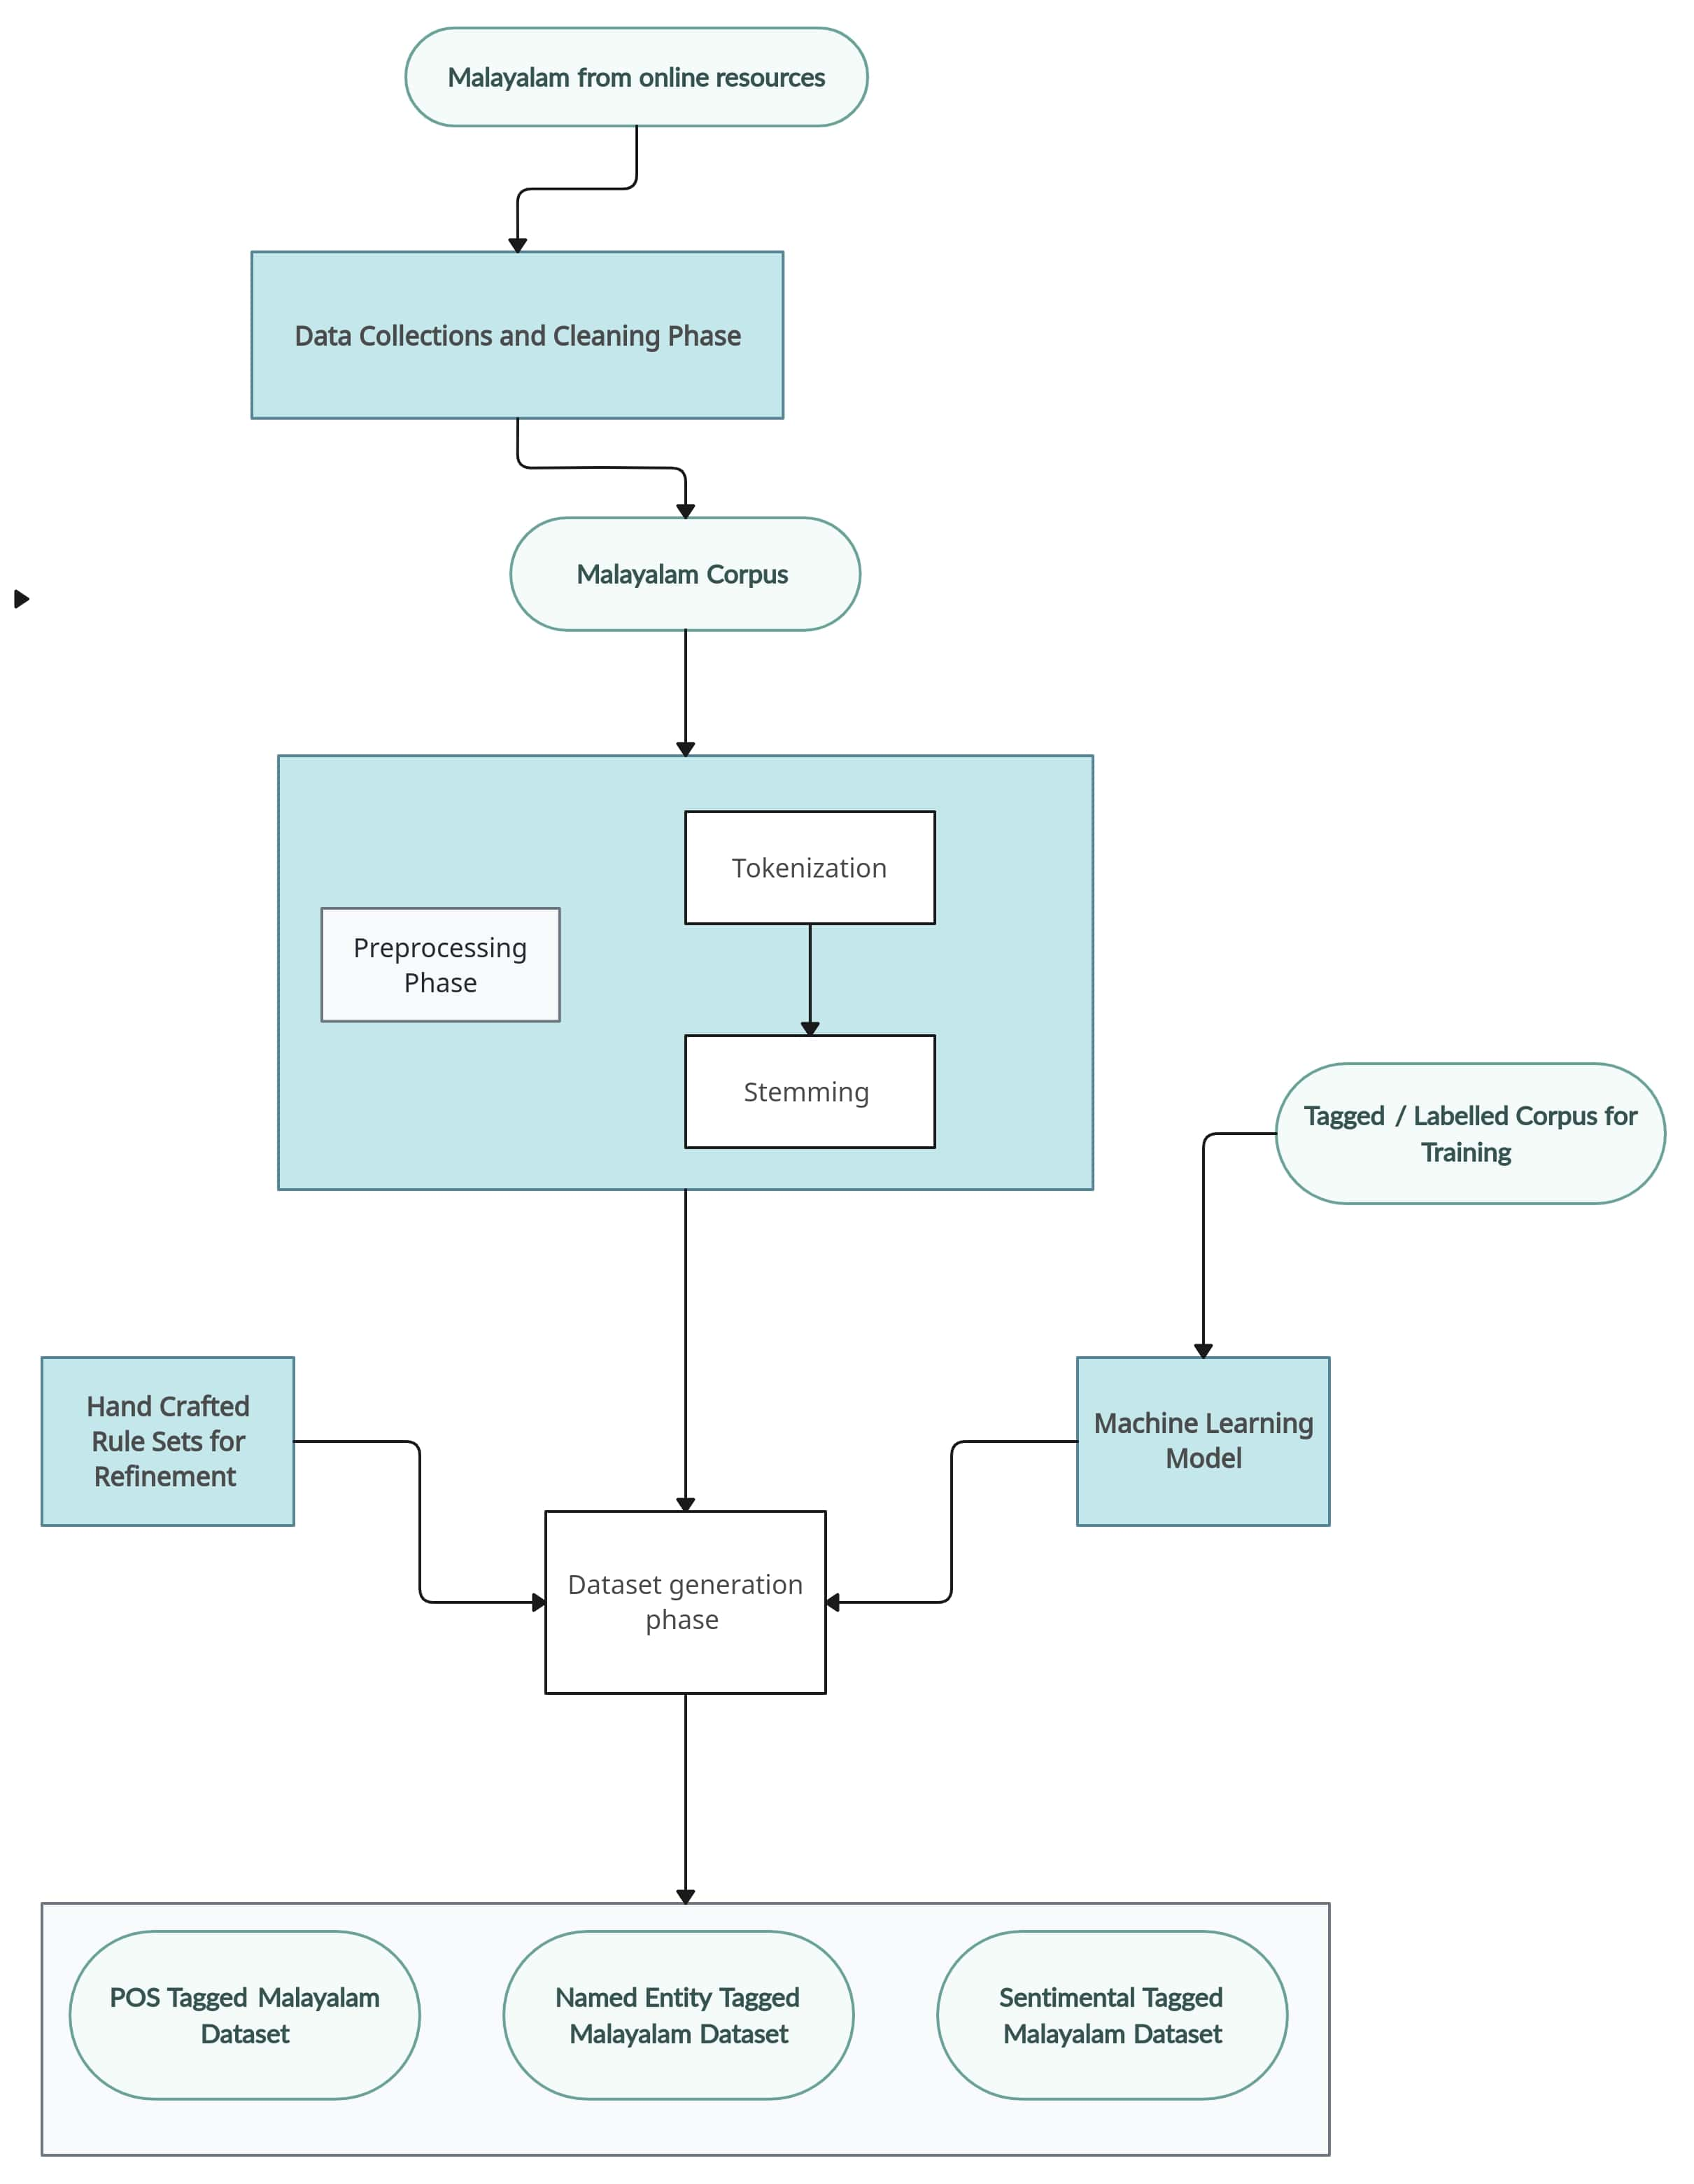
\includegraphics[width=12cm]{./system_design.jpg}
		\caption{System design}
	\end{figure}
	\subsection{Product Functions}
	\paragraph\
	Major Functions of the Malayalam Parser:
	\begin{itemize}
		\item  Parse and analyze Malayalam language text to identify linguistic components such as words,
		phrases, and sentences.
		\item Determine grammatical structure, syntax, and semantics of Malayalam sentences to facilitate
		accurate linguistic analysis.
		\item Provide functionality for part-of-speech tagging, syntactic parsing, and semantic analysis
		tailored for the Malayalam language.
		\item Support for handling compound words, inflections, and variations in word forms commonly
		found in Malayalam text.
		\item Generation of a part-of-speech tagged dataset, named entity dataset, and sentimental tagged
		dataset, contributing to the advancement of language processing technologies in Malayalam
	\end{itemize}
    \subsection{Operating Environment}
    For creating the Malayalam Parser, the operating environment encompasses the following specifications:
    \newline
    \textbf{Hardware Platform}
    \begin{itemize}
    	\item The software should be compatible with standard computing hardware commonly used for
    	software development and deployment.
    	\item Minimum hardware requirements include a modern processor (e.g., Intel Core i5 or equivalent),
    	sufficient RAM (at least 4GB), and available storage space for software installation and data
    	processing.
    \end{itemize}
    \textbf{Operating System and Versions}
    \begin{itemize}
    	\item The software should be compatible with popular operating systems used for software development
    	and deployment, including Windows, MacOS, and Linux distributions.
    	\item Specific operating system versions supported include:
    	\newline
    	Windows 10 or later
    	\newline
    	MacOS 10.13 High Sierra or later
    	\newline
    	Ubuntu 18.04 LTS or later
    \end{itemize}
    \textbf{Software Components and Applications}
    \begin{itemize}
    	\item The Malayalam Parser may require integration with various software components and applications
    	for development, testing, and deployment purposes.
    	\item Development tools such as Python (version 3.6 or later), Java Development Kit (JDK),
    	or other programming languages and frameworks suitable for NLP development may be
    	necessary.
    	\item Libraries and frameworks for natural language processing, such as NLTK (Natural Language
    	Toolkit), spacey or TensorFlow, may be utilized.
    	\item Database systems such as SQLite, PostgreSQL, or MongoDB may be employed for data
    	storage and retrieval if necessary.
    \end{itemize}
	
	\subsection{Design and Implementation Constraints}
	\paragraph\
	The development of the Malayalam Parser is subject to various constraints and limitations, including:
	\begin{itemize}
	\item \textbf{Hardware Limitations:} The software must be optimized to operate within hardware limitations,
	including timing and memory constraints. Performance optimizations are crucial to ensure
	efficient operation across different hardware configuration.
	\item \textbf{Integration with External Systems:} The parser must support standard interfaces and data
	formats for interoperability with other language processing tools or databases. Ensuring
	smooth integration is a technical requirement.
	\item \textbf{Language Requirements:} The Malayalam Parser must be designed and implemented to
	meet the linguistic complexities of the Malayalam language. This includes handling unique
	grammar rules, character encoding, and text processing requirements inherent to Malayalam.
	\item \textbf{Character Encoding and Localization:} Proper handling of character encoding specific
	to Malayalam and localization considerations are crucial. The parser should accurately
	interpret and process Malayalam characters.
	\item \textbf{Security Considerations:} Security measures such as encryption, access control, and data
	integrity must be incorporated into the design and implementation of the Malayalam Parser
	to safeguard against security threats and vulnerabilities.
	\item \textbf{Design Conventions and Programming Standards:} Adherence to design conventions,
	programming standards, and coding guidelines is paramount. Developers must follow established
	best practices and organizational standards to ensure maintainability, readability, and consistency
	of the codebase.
\end{itemize}

\subsection{Assumptions and Dependencies}

\begin{enumerate}
	\item  \textbf{Third-Party or Commercial Components:} It is assumed that the development of the
	Malayalam Parser will rely on third-party or commercial components. The project is intended
	to be developed from existing models, without significant dependencies on pre-existing
	software solutions or proprietary libraries.
	\item \textbf{Development Environment:} The assumption is made that the development environment
	for the Malayalam Parser will be properly configured and equipped with necessary tools,
	including programming languages, development frameworks, and version control systems.
	\item \textbf{Operating Environment:} It is assumed that the operating environment for testing and
	deployment of the Malayalam Parser will meet the specified requirements, including compatibility
	with supported operating systems and hardware configurations.
	\item \textbf{Constraints and Limitations:} The project assumes that constraints and limitations identified
	in the SRS, such as corporate policies, regulatory requirements, and hardware limitations,
	will be properly addressed and accounted for during the development process.
	\item \textbf{External Dependencies:} The project does anticipate reliance on external dependencies or
	reused software components from other projects. Any dependencies arising during development
	will be clearly documented and managed accordingly.
	\item \textbf{Availability of Resources:} It is assumed that the necessary resources, including human
	resources, budget allocation, and development timelines, will be available and allocated
	appropriately to support the successful development and completion of the Malayalam Parser
	project.
\end{enumerate}
	\section{External Interface Requirements}
	\subsection{User Interfaces}
	\paragraph\
	The project has the potential to be utilized in various future applications, particularly in educational
	tools designed for teaching purposes. Additionally, it can serve as a foundation for developing apps focused on language learning, text analysis, and speech recognition. This versatility opens
	up opportunities for creating interactive and innovative tools that cater to different learning styles
	and linguistic analysis needs. By leveraging the project’s capabilities, we can create user-friendly
	applications that enhance the learning and analysis experience for users. These applications can
	play a significant role in promoting the Malayalam language and its usage in various contexts.
	 
	\subsection{Hardware Interfaces}
	\paragraph\
	The software interacts with the hardware components of the system through various interfaces,
	each with specific communication protocols. It communicates with the CPU to execute algorithms,
	process data, and manage computational tasks, utilizing the CPU’s instruction set architecture.
	The software uses RAM for temporary storage of linguistic data, parsing results, and intermediate
	processing steps, managing memory efficiently for complex linguistic analyses. For long-term
	storage, the software reads and writes data to the storage device, employing file systems for dataset
	management and data integrity. Optionally, the software can access external datasets, online
	resources, or collaboration tools through a network interface, using standard networking protocols
	such as HTTP or FTP for data exchange. User interaction and data visualization are facilitated
	through input/output devices such as keyboards, mouse, and monitors, utilizing standard interfaces
	for user input and output display.
	
	\subsection{Software Interfaces}
	\paragraph\
	The Malayalam parser integrates with various software components, including databases such as
	SQLite, PostgreSQL, and MongoDB for data storage and retrieval. It is designed to run on popular
	operating systems like Windows 10 or later, MacOS 10.13 High Sierra or later, and Ubuntu 18.04
	LTS or later. Development and NLP tasks are facilitated by Python (version 3.6 or later) along with
	libraries like NLTK, Spacy, and TensorFlow. These tools aid in implementing NLP algorithms
	and processing linguistic data. The system may also include integrated commercial components
	for specific functionalities, each with its own data formats, configurations, and communication
	protocols. To ensure consistent data sharing, the system may implement global data areas or
	standardized data formats, depending on the software components involved. Detailed application programming interface (API) protocols should be referenced for precise communication details.
	
	\subsection{Communication Interfaces}
	\paragraph\
	The software requires communication functions for fetching inputs from websites, email, and
	network server communications. It needs to support standard email protocols like SMTP for
	sending emails, following MIME standards for message formatting. For web scraping, it should
	interact with web servers using HTTP or HTTPS for secure communication, and handle HTML
	parsing for extracting data from web pages. Network server communication may require protocols
	like FTP or SFTP for file transfers, adhering to communication standards for compatibility and
	security. Secure protocols such as SMTPS, SFTP, or TLS should be used for data transmission,
	with defined data transfer rates and synchronization mechanisms for efficiency. 
	
    
	
	\section{System Features}
	\paragraph\ 
	The system features for the Malayalam Parser are organized to highlight the major services provided
	by the product:
	\begin{enumerate}
		\item  \textbf{Text Parsing:} The parser breaks down Malayalam language text into its constituent components
		such as words, phrases, and sentences.
		\item \textbf{Grammatical Analysis:} It identifies the parts of speech, syntactic structure, and grammatical
		relationships within Malayalam sentences.
		\item \textbf{Semantic Analysis:} The system determines the meaning and interpretation of Malayalam
		text, capturing semantic relationships between words and phrases.
		\item \textbf{Part-of-Speech Tagging:} Each word in a Malayalam sentence is assigned appropriate part-of-speech tags, indicating its grammatical function.
		\item \textbf{Syntactic Parsing:} It analyzes the syntactic structure of Malayalam sentences, identifying
		constituents and their hierarchical relationships.
		\item \textbf{Error Handling:} Mechanisms are in place to detect and handle errors or inconsistencies in
		input Malayalam text, ensuring parsing reliability.
		\item \textbf{ Customization and Extension:} Users can customize and extend the parser with custom
		linguistic rules, dictionaries, or algorithms for domain-specific parsing tasks.
	\end{enumerate}
	
	\subsection{Parsing Malayalam Text}
	
	\subsubsection{Description and Priority}
	\paragraph\
	This feature involves analyzing and understanding the linguistic structure of Malayalam text,
	including sentence segmentation, word tokenization, and part-of-speech tagging. It is of high
	priority as it forms the core functionality of the system.
	
	\subsubsection{Stimulus/Response Sequences}
	
	Stimulus: User inputs a Malayalam text.
	\newline
	Response: The system parses the text, segments sentences, tokenizes words, and tags parts of
	speech.
	
	\subsubsection{Functional Requirements}
	\begin{enumerate}
		\item  The system shall be able to segment sentences in Malayalam text based on punctuation marks
		and grammatical rules.
		\item The system shall tokenize words in Malayalam text, considering compound words and affixes.
		\item The system shall tag each word in Malayalam text with its respective part of speech (e.g.,
		noun, verb, adjective).
		\item The system shall handle variations in spelling and word forms commonly found in Malayalam
		text.
		\item The system shall provide error messages for invalid inputs or unsupported characters.
		\item The system shall process text efficiently, aiming for a parsing speed of at least X characters
		per second.
		\item The system shall be able to handle text inputs of up to Y characters in length.
	\end{enumerate}
	
	
	\subsection{Lemmatization and Morphological Analysis}
	\subsubsection{Description and Priority}
	\paragraph\
	This feature involves performing lemmatization to identify the base form of words and morphological
	analysis to understand the grammatical properties of words. It is of high priority as it enhances the
	accuracy of language analysis.
	
	\subsubsection{Stimulus/Response Sequences}
	Stimulus: User inputs a Malayalam word
	\newline
	Response: The system lemmatizes the word and performs morphological analysis to determine its
	grammatical properties.
	
	\subsubsection{Functional Requirements}
	
	\begin{enumerate}
		\item  The system shall lemmatize Malayalam words to identify their base forms.
		\item The system shall analyze the morphology of Malayalam words to determine their grammatical
		properties.
		\item The system shall handle variations in word forms and inflections commonly found in Malayalam.
		\item The system shall provide error messages for invalid inputs or unsupported characters.
		\item The system shall process words efficiently, aiming for a lemmatization speed of at least X
		words per second.
		\item The system shall be able to handle word inputs of up to Y characters in length.
	\end{enumerate}
	
	\subsection{Dependency Parsing}
	\subsubsection{Description and Priority}
	\paragraph\
	Dependency parsing involves identifying the syntactic dependencies between words in a sentence,
	which is crucial for understanding the relationships within the sentence. It is of high priority as it
	provides valuable linguistic information for further analysis.
	
	\subsubsection{Stimulus/Response Sequences}
	Stimulus: User inputs a Malayalam sentence.
	\newline
	Response:The system parses the sentence to identify syntactic dependencies between words.
	
	
	\subsubsection{Functional Requirements}

	\begin{enumerate}
		\item  The system shall parse Malayalam sentences to identify syntactic dependencies between
		words.
		\item The system shall generate dependency trees that represent the syntactic structure of parsed
		sentences.
		\item The system shall handle complex sentence structures and dependencies between words.
		\item The system shall provide error messages for invalid inputs or unsupported characters.
		\item The system shall process sentences efficiently, aiming for a parsing speed of at least X
		sentences per second.
		\item The system shall be able to handle sentence inputs of up to Y characters in length.
	\end{enumerate}
	\subsection{Syntax Tree Generation}
	\subsubsection{Description and Priority}
	\paragraph\
	Syntax tree generation involves creating syntax trees that represent the grammatical structure of
	sentences. It is of high priority as it provides a visual representation of the sentence’s structure,
	aiding in linguistic analysis.
	
	\subsubsection{Stimulus/Response Sequences}
	Stimulus: User inputs a Malayalam sentence.
	\newline
	Response: The system analyzes the sentence’s grammatical structure and generates a syntax tree.
	
	\subsubsection{Functional Requirements}
	\begin{enumerate}
		\item  The system shall generate syntax trees for Malayalam sentences based on their grammatical
		structure.
		\item The system shall use standard tree representation formats (e.g., Penn Treebank format) for
		generated syntax trees.
		\item The system shall handle complex sentence structures, including coordination and subordination.
		\item The system shall provide options for visualizing syntax trees, such as tree diagrams or textual
		representations.
		\item The system shall process sentences efficiently, aiming for a tree generation speed of at least
		X trees per second.
	\end{enumerate}
	
	\subsection{Semantic Analysis}
	\subsubsection{Description and Priority}
	\paragraph\
	Semantic Analysis is a critical feature of the system, with a high priority. It involves determining
	the meaning and interpretation of Malayalam text, capturing semantic relationships between words
	and phrases.
	
	\subsubsection{Stimulus/Response Sequences}
	Stimulus: User inputs Malayalam text for analysis.
	\newline
	Response: The system processes the text to extract meaning and semantic relationships.
	
	\subsubsection{Functional Requirements}
	\begin{enumerate}
		\item  The system shall identify subject-verb-object relationships in Malayalam sentences.
		\item It shall detect and interpret negation, conjunctions, and other semantic features in the text.
		\item The system shall extract key concepts and entities from the text.
		\item It shall handle ambiguous phrases and provide contextually appropriate interpretations.
		\item The system shall support the identification of sentiment and emotions expressed in the text.
		\item It shall provide an API or interface for developers to access the semantic analysis results.
		\item The system shall handle errors gracefully, providing informative messages for incorrect
		inputs.
		\item It shall process text efficiently, aiming for a response time of less than 1 second for short to
		medium-length texts.
		\item It shall be able to process text with a wide range of vocabulary and language complexity
		levels, including formal and informal language variants.
	\end{enumerate}
	
	\subsection{Part-of-Speech tagging}
	\subsubsection{Description and Priority}
	\paragraph\
	Part-of-Speech Tagging is a critical feature of the system, with a high priority. It involves assigning
	grammatical tags to words in Malayalam sentences, indicating their syntactic role and category.
	
	\subsubsection{Stimulus/Response Sequences}
	Stimulus: User inputs Malayalam text for analysis.
	\newline
	Response: The system processes the text and assigns appropriate part-of-speech tags to each word.
	
	\subsubsection{Functional Requirements}
	\begin{enumerate}
		\item  The system shall identify the part of speech for each word in the input Malayalam text.
		\item It shall handle compound words and inflected forms, assigning appropriate tags based on
		their usage in context.
		\item The system shall support standard part-of-speech tag sets for Malayalam, ensuring compatibility
		with existing linguistic resources.
		\item It shall provide an option to output the tagged text in a readable format for users.
		\item The system shall be able to handle texts with varying levels of complexity and vocabulary.
		\item It shall provide an API or interface for developers to access the tagged text and integrate it
		into their applications.
		\item The system shall handle errors gracefully, providing informative messages for incorrect
		inputs.
	\end{enumerate}
	
	\subsection{Performance Requirements}
	\subsubsection{Description and Priority}
	\paragraph\
	Performance optimization involves improving the efficiency and speed of the system. It is of low
	priority as it is desirable but not critical for basic functionality.
	\subsubsection{Stimulus/Response Sequences}
	Stimulus: System performance falls below specified thresholds.
	\newline
	Response: The system implements optimization techniques to improve performance
	
	\subsubsection{Functional Requirements}
	\begin{enumerate}
		\item  The system shall monitor performance metrics, such as processing speed and resource usage.
		\item The system shall identify performance bottlenecks and areas for improvement.
		\item The system shall implement optimizations, such as algorithmic improvements or resource
		management strategies, to enhance performance.
		\item The system shall provide configuration options for adjusting performance settings based on
		user needs
	\end{enumerate}
	
	
	\section{Other Nonfunctional Requirements}
	\subsection{Performance Requirements}
	
	\subsubsection{Parsing Malayalam Text}
	\paragraph\
	Rationale: Parsing text should be fast to provide timely analysis for user interactions or batch
	processing.
	\newline
	Requirement: The system should be able to parse Malayalam text at a rate of at least 1000
	characters per second.
	
	\subsubsection{Lemmatization and Morphological Analysis}
	\paragraph\
	Rationale: Lemmatization and morphological analysis are core linguistic processes that should not
	introduce significant delays.
	\newline
	Requirement: The system should be able to perform lemmatization and morphological analysis for
	at least 100 words per second.
	
	\subsubsection{Dependency Parsing}
	\paragraph\
	Rationale: Dependency parsing is computationally intensive but crucial for understanding sentence
	structures.
	\newline
	Requirement: The system should be able to perform dependency parsing for at least 50 sentences
	per second.
	
	\subsubsection{Syntax Tree Generation}
	\paragraph\
	Rationale: Syntax tree generation requires complex computations and should be efficient for real-time applications.
	\newline
	Requirement: The system should be able to generate syntax trees for at least 20 sentences per
	second.
	
	\subsubsection{Semantic Analysis}
	\paragraph\
	Rationale: Semantic analysis involves processing text to understand its meaning, requiring significant
	computational resources. Efficient performance is crucial for real-time or near real-time applications,
	such as chatbots or text summarization systems.
	\newline
	Requirement: The system should be able to perform semantic analysis for a minimum of 1000
	words per second, ensuring timely and responsive processing for various use cases.
	
	\subsubsection{Part-of-Speech tagging}
	\paragraph\
	Rationale: Part-of-speech tagging is a fundamental task in natural language processing, providing
	essential grammatical information about words in a sentence. Efficient tagging is necessary for
	various downstream tasks such as parsing, machine translation, and information extraction.
	\newline
	Requirement: The system should be able to perform part-of-speech tagging for a minimum of 1000
	words per second, ensuring fast and responsive tagging for different text lengths and complexities.
	
	\subsubsection{Performance Optimization}
	\paragraph\
	Rationale: Performance optimization ensures that the system meets its performance requirements
	under varying loads and conditions.
	\newline
	Requirement: The system should implement optimization strategies to maintain performance levels
	even under heavy loads, ensuring that response times do not exceed specified thresholds.
	

	 
   \subsection{Safety Requirements}
   \paragraph\
   Loss, Damage, or Harm Concerns: The product must ensure user and property safety, preventing
   physical harm or damage. It must also safeguard sensitive data from unauthorized access.
   \newline 
   Actions to be Taken: The product should provide clear instructions and warnings to prevent misuse
   or accidental damage. Regular maintenance and updates are crucial for safe operation.
   \newline
    Actions to
   be Prevented: Unauthorized modifications and operations that could lead to data loss or corruption
   should be prevented.
   \newline
   External Policies or Regulations: Compliance with safety standards and regulations is essential,
   including guidelines from regulatory bodies and industry standards organizations.
   \newline
   Safety Certifications: Obtaining safety certifications demonstrates compliance with standards and
   builds user trust in the product’s safety.
   
   \subsection{Security Requirements}
   \paragraph\
   The system must prioritize the security and privacy of the data used or created by the system.
   It should implement robust measures to prevent unauthorized access, disclosure, or modification
   of sensitive information, such as annotated dataset files. User identity authentication should be
   incorporated to verify the identity of users accessing the system, ensuring that only authorized
   users can access or modify the dataset files. The system must comply with external policies and
   regulations regarding security and privacy issues, adhering to guidelines set by regulatory bodies
   or industry standards organizations. Obtaining security and privacy certifications is essential to
   demonstrate compliance with these standards, reassuring users of the parser’s commitment to data
   security and privacy protection.
   
   \subsection{Software Quality Attributes}
   \paragraph\
   The Malayalam parser for dataset creation must prioritize correctness and reliability, ensuring
   accurate parsing and consistent results. Maintainability is crucial for easy updates, while usability
   requires an intuitive interface. Portability enables the parser to run on different platforms, and
   interoperability allows integration with other NLP components. Testability ensures thorough testing,
   and adaptability allows for evolving requirements. These characteristics collectively ensure the
   parser’s efficiency, effectiveness, and adaptability.
   
	
	
	\chapter{System Architecture and Design}
	\section{System Overview }
	
	
	
	\paragraph\
	The aim of the project to develop a Malayalam parser is to create a system that can effectively process Malayalam text for tasks such as sentiment analysis, named entity recognition, and part-of-speech (POS) tagging. The process begins with data collection, where Malayalam text is gathered from online sources using web scraping techniques. This collected text is then cleaned to remove any irrelevant information, errors, or special characters.
	\newline
	Language filtering is applied in the cleaning phase to ensure the text is in Malayalam. Following data cleaning, the text undergoes preprocessing, which includes tokenization to break the text into individual words or tokens. Stemming is then applied to reduce inflected words to their base form, simplifying the text for analysis. A crucial step is building a training corpus of preprocessed Malayalam text labeled with the desired information, such as sentiment labels, named entities, and part-of-speech tags. Features are extracted from the preprocessed text and serve as inputs to the machine learning model. A suitable machine learning model is selected and trained on the extracted features and labeled training data. The model's performance is evaluated on a separate set of data to assess its accuracy and effectiveness on new, unseen data. Finally, the trained model is used to process new Malayalam text, tagging it with sentiment labels, named entities, part-of-speech tags, or other relevant information. Linguists can add custom rules to refine the model's output for better accuracy. 
	\begin{figure}[H]
		\centering
		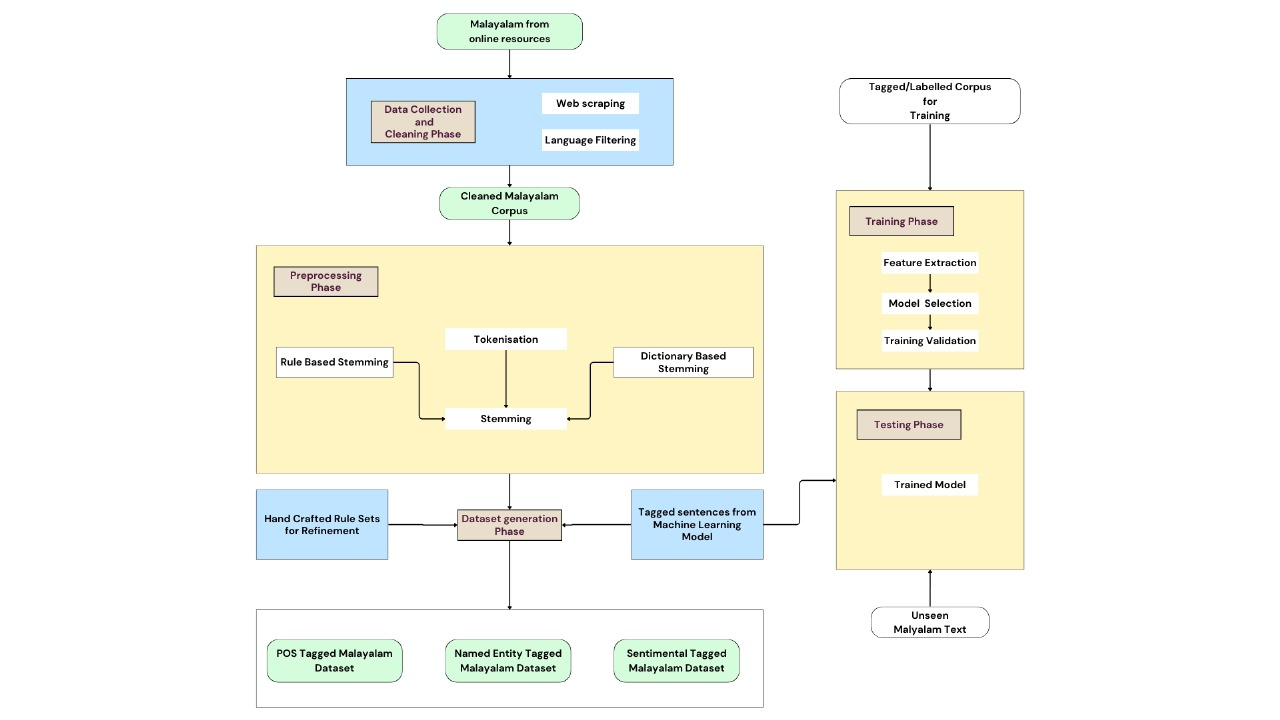
\includegraphics[width=19cm]{./architecture.jpg}
		\caption{Architecture diagram}
	\end{figure}
	
	\section{Dataset identified}
	\paragraph\ 
	This section describes the data source used in the project. Brief its properties and refer it to
	the appropriate location. Sample subsets of the dataset can be highlighted.
	
	
	
	\section{Proposed Methodology/Algorithms}
	\paragraph\ 
	This section describes in detail the methodologies or algorithms associated with your work.
	Algorithms should be written in appropriate format.
	
	\section{User Interface Design}

	\begin{figure}[H]
		\centering
		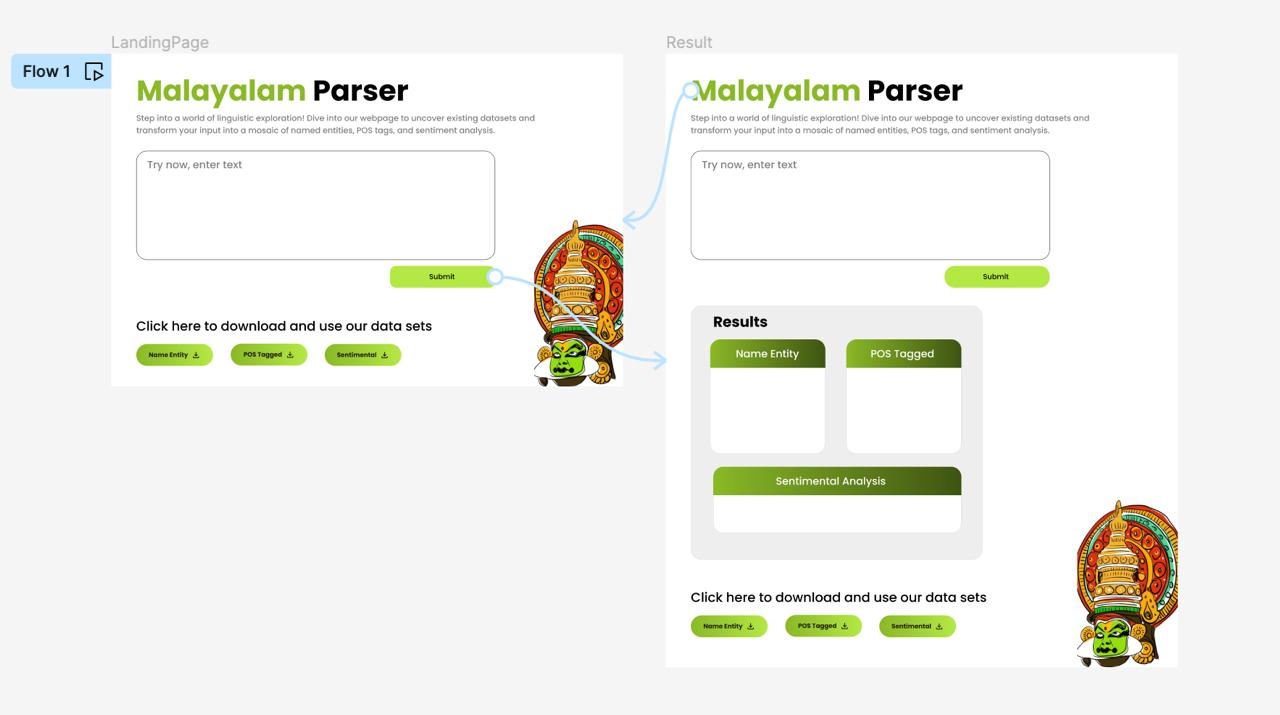
\includegraphics[width=16cm]{./ui.jpg}
		
	\end{figure}
	
	\begin{figure}[H]
		\centering
		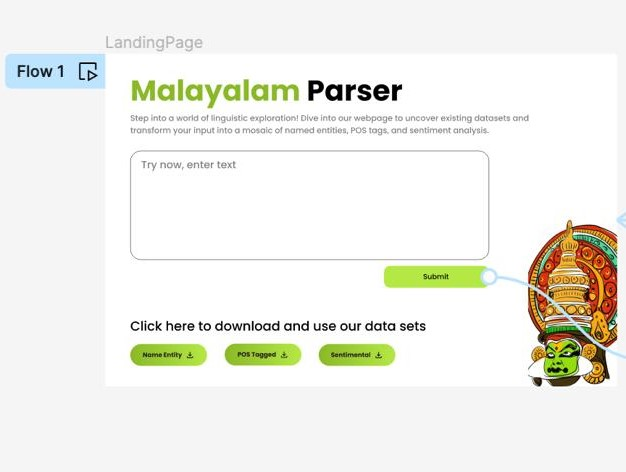
\includegraphics[width=14cm]{./landing.jpg}
		\caption{Landing page}
	\end{figure}
	
	\begin{figure}[H]
		\centering
		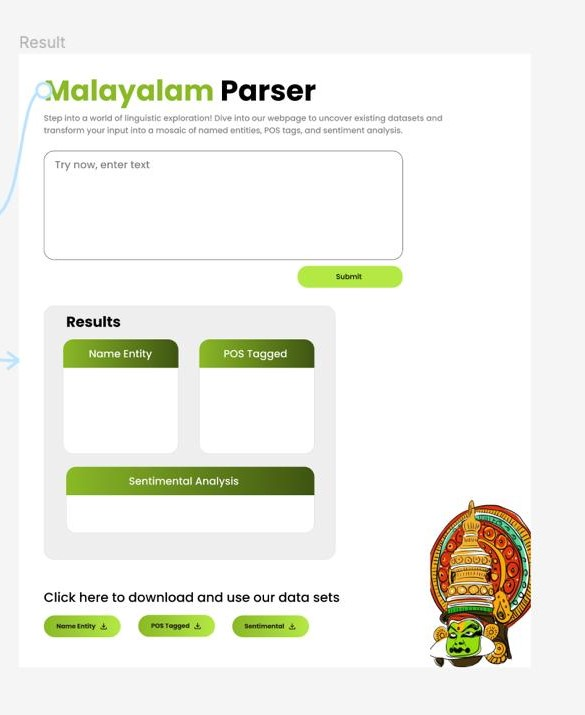
\includegraphics[width=14cm]{./result.jpg}
		\caption{Result page}
	\end{figure}
	
	
	
	
	
	\section{Description of Implementation Strategies}
	\paragraph\
	The implementation strategies for the project are as follows:
	\begin{itemize}
		\item Data Acquisition and Cleaning:
		\begin{enumerate}
			\item  Web Scraping:
			\begin{itemize}
				\item Utilize libraries like BeautifulSoup or Scrapy (Python) to scrape
				relevant Malayalam websites.
				\item Define target URLs and develop scraping logic for text extraction.
				\item Implement techniques to handle pagination or dynamic content loading
				(if applicable).
			\end{itemize}
			
			\item Language Filtering:
			\begin{itemize}
				\item  Implement language detection using libraries like langdetect or
				textblob (Python) to identify non-Malayalam text.
				\item Set a threshold or confidence score to filter out content below a certain
				level of Malayalam probability.
			\end{itemize}
			
		\end{enumerate}
		\item Data Preprocessing:
		\begin{enumerate}
			\item  Tokenization:
			Choose a suitable tokenization method (word-based, sentence-based,
			etc.) using libraries like NLTK or spaCy (Python).
			
			\item Handling Non-Textual Elements:
			Develop logic for managing emojis or other non-textual elements (e.g.,
			removal, special token representation).
			
			\item Stop Word Removal:
			Implement stop word removal based on a created or located
			Malayalam stop word list.
			\item Stemming or Lemmatization:
			Use libraries like NLTK or spaCy for stemming (reducing words to root
			forms) or lemmatization (finding dictionary base forms).
			Explore specific stemming/lemmatization algorithms if necessary for
			Malayalam.
			
		\end{enumerate}
		
		\item Sentiment Analysis:
		\begin{enumerate}
			\item  Model Selection (if applicable):
			Consider factors like data size, desired accuracy, and computational
			resources when choosing a model (e.g., Logistic Regression, Naive
			Bayes, SVM, RNNs).
			\item Data Splitting (if applicable):
			Split the preprocessed data into training, validation, and testing sets for
			model development.
			
			\item Model Training and Tuning (if applicable):
			Implement hyperparameter tuning to optimize model performance
			during training.
			\item Evaluation (if applicable):
			Evaluate the trained sentiment analysis model's performance on the unseen testing data set.
			Analyze the results and identify areas for improvement in data quality
			or model architecture.
		\end{enumerate}
		
		\item Additional Considerations:
		\begin{enumerate}
			\item  Data Storage and Management: Consider implementing data loading/saving
			functions for various formats (text files, CSV, etc.) if needed for further
			analysis.
			\item Version Control: Utilize a version control system (e.g., Git) to track code
			changes and facilitate collaboration.
			\item Testing: Implement unit tests for critical functions and integration tests to
			ensure the entire NLP pipeline functions as expected.
			\item Logging: Implement logging functionalities to track code execution progress
			and identify potential issues.
		\end{enumerate}
		
	\end{itemize}
	
	\section{Module Division}
	\begin{itemize}
	\item Module 1: Data Collection and Preprocessing (Team Member 1: Mohammed Basil)
	\begin{itemize}
	\item Data Acquisition: Collect Malayalam text data from various sources such as websites, documents, or databases.
	\item Data Cleaning: Preprocess collected data to remove noise, inconsistencies, or irrelevant information.
	\item Language Identification: Determine the language of the text to ensure only Malayalam language text is processed.
	\item Tokenization: Divide the preprocessed text into individual tokens or words following Malayalam language rules and conventions.
\end{itemize}
	\item Module 2: UI Design (Team Member 2: Godwin Gino)
	\begin{itemize}
	\item User Interface Components: Design and implement user interface elements such as input fields, buttons, text areas, and output displays.
	\item Interaction Logic: Manage user interactions, including event handling, input validation, and feedback mechanisms.
	\item Layout and Styling: Define layout structure, visual design, and styling for an intuitive and aesthetically pleasing user experience.
\end{itemize}
	\item Module 3: Rule Set Generation (Team Member 3: Fathima Jennath)
	\begin{itemize}
	\item Rule Extraction: Extract linguistic rules and patterns from annotated data or linguistic resources specific to Malayalam language parsing.
	\item Rule Representation: Represent extracted rules in a formal format suitable for integration into the parsing module.
	\item Rule Validation and Optimization: Validate generated rules for accuracy and completeness, optimizing them for efficient parsing of Malayalam text.
\end{itemize}
	\item Module 4: Machine Learning and Dataset Generation (Team Member 4: Gautham C Sudheer)
	\begin{itemize}
	\item Dataset Collection and Annotation: Acquire or generate a dataset of Malayalam text samples, annotating them with linguistic information.
	\item Feature Extraction: Identify relevant features or attributes from the annotated dataset using techniques like bag-of-words or word embeddings.
	\item Model Training and Evaluation: Train machine learning models for tasks such as part-of-speech tagging or named entity recognition, evaluating their performance using metrics like accuracy.
\end{itemize}
\end{itemize}
	\section{Work Schedule - Gantt Chart}
	
	\begin{figure}[H]
		\centering
		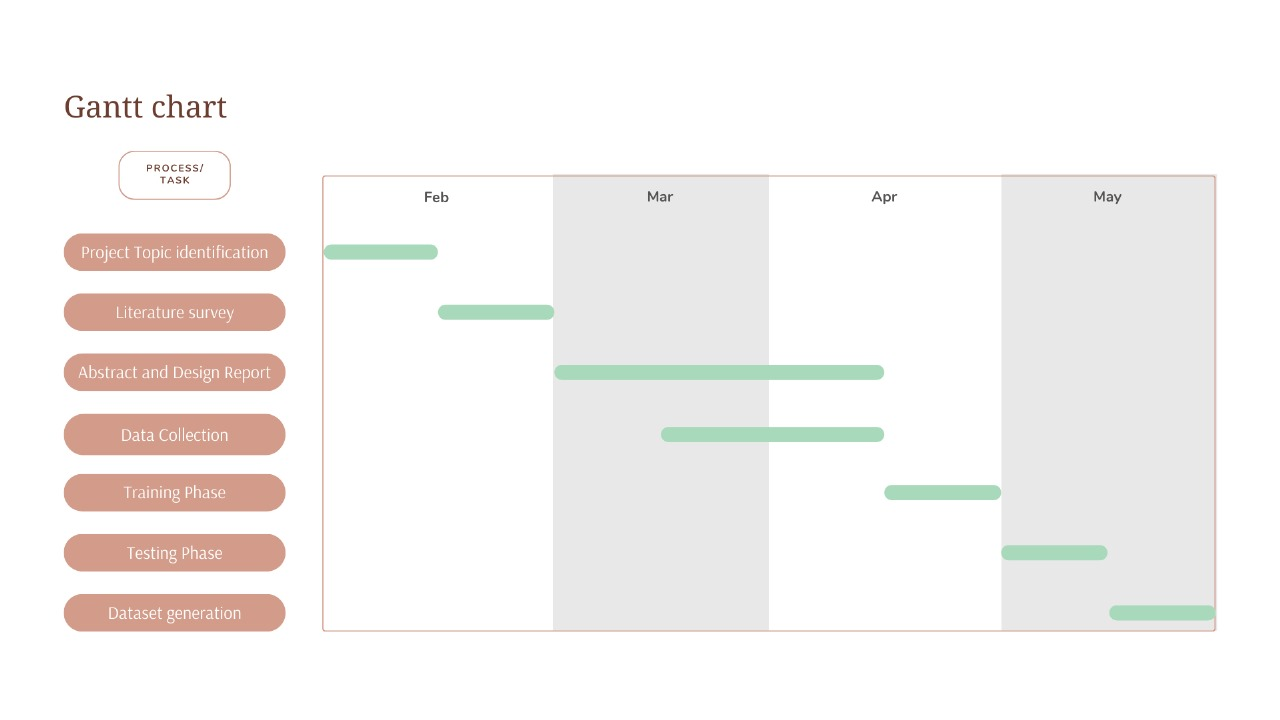
\includegraphics[width=18cm]{./ganttchart.jpg}
		\caption{Work Schedule-Gantt chart}
	\end{figure}
	
	\paragraph\ 
	
	
	
	%	\chapter{Results and Discussions}
	
	
	%	\section{Overview}
	%	\paragraph\
	%	This section describes the overall results achieved in terms of the end results, quantitative	results and further analysis. One paragraph of textual description is expected.
	
	
	%	\section{Testing}
	%	\paragraph\
	
	%	For a webapp/database project, screenshots of results in chronological order can be added	in this section. Other types of projects also can have this section with less length.
	
	
	%	\section{Quantitative Results}
	%	\paragraph\
	%	The quantitative results of the project (eg- numerical values like accuracy, precision, rmse,	confusion matrix etc ) can be supplemented in this section. Important note is textual description of all results is mandatory. Give appropriate titles for the tabular results.
	
	
	%	\section{Graphical Analysis}
	%	\paragraph\
	%	The graphical analysis of the project can be given in this section. Choose your graph	representation in accordance with your project. Important note is textual description of allvresults is mandatory. Give appropriate titles for the graphical results. In this section, comparison of your results with other paper titles mentioned in Chapter 2 are also encouraged.
	
	
	%	\section{Discussion}
	%	\paragraph\
	%	This section describes a summary of the results. You are also welcome to substantiate the reason behind your results or also the deviation of the results.
	
	%	\chapter{Conclusion}
	
	
	%	\section{Conclusion}
	%	\paragraph\
	%	This section describes the conclusion of the project in one page. Write one or two paragraphs.
	
	
	%	\section{Future Scope}
	%	\paragraph\
	%	In this section outline the future scope/extensions possible in the project in four or five	sentences.
	
	%	\newpage
	%	\normalsize{}
	
	%	\chapter*{List of Publications}
	%	\addcontentsline{toc}{chapter}{Publications}
	%	\begin{enumerate}
		%		\item Publication 1
		%		\item Publication 2
		%	\end{enumerate}
	
	
	%	\clearpage
	%	\renewcommand{\bibname}{References} 
	%	\addcontentsline{toc}{chapter}{References}
	
	\begin{thebibliography}{99}
		\bibitem a Asopa, S., and Sharma, N. (2021) A Hybrid Parser Model for Hindi Language. Indian Journal of Computer Science and Engineering (IJCSE), Vol. 12(1).
		\bibitem b Chen, D., and Manning, C. D. (2014). A Fast and Accurate Dependency Parser using Neural Networks. Proceedings of the 2014 Conference on Empirical Methods in Natural Language	Processing (EMNLP).
		\bibitem c Nair, L. R. (2013). Language Parsing and Syntax of Malayalam Language. 2nd International
		Symposium on Computer, Communication, Control and Automation (3CA 2013).
		\bibitem d Berger, A. L., Della Pietra, V. J., and Della Pietra, S. A. (1996). A Maximum Entropy
		Approach to Natural Language Processing. Association for Computational Linguistics, Vol
		22(1).
		\bibitem e Mestry, A., Shende, S., Mahadik, A., and Virnodkar, S. (2014). A Parser: Simple English
		Sentence Detector and Correction. International Journal of Engineering Research and Technology
		(IJERT).
		\bibitem f Sethi, N., Agrawal, P., Madaan, V., and Singh, S. K. (2016). A Novel Approach to Paraphrase
		Hindi Sentences using Natural Language Processing. Indian Journal of Science and Technology,
		Vol 9(28).
		\bibitem g Smith, D. A., and Eisner, J. (2008). Dependency Parsing by Belief Propagation. Proceedings
		of the 2008 Conference on Empirical Methods in Natural Language Processing, Page 145-
		156.
		
		\bibitem h Bharati, A., Kulkarni, A., and Chaudhury, S. (2007). English Parsers: Some Information-
		based Observations.
		
		\bibitem i Jayan, J. P., and R, R. (2009). A Morphological Analyzer for Malayalam - A Comparison of
		Different Approaches. International Journal of Computer Science and Information Technology.
		Vol 2(2), Page 155-160.
		
		\bibitem j Vaidya, A., Choi, J. D., Palmer, M., and Narasimhan, B. (2011). Analysis of the Hindi
		Proposition Bank using Dependency Structure. Proceedings of the Fifth Law Workshop
		(LAW V), Page 21-29.
		\bibitem k Rajan, M., T.S, R., and Bhojane, V. (2014). Information Retrieval in Malayalam Using Natural
		Language Processing. International Journal of Scientific and Engineering Research, Vol 5(6)
		\bibitem l Rajan, M., Thirumalai, R., and Kumar, V. (2006). Development of a Tamil Parser using
		Natural Language Processing Techniques. A survey of the state of the art in tamil language
		technology Vol 6(10).
		\bibitem m Venkatesh, R., Kumar, S., and Arumugam, P. (2014). Building a Lexical Analyzer for Tamil
		Texts using NLP Approaches. 2014 International Conference on Advances in ICT for Emerging
		Regions (ICTer).
		\bibitem n Thavareesan, S., and Mahesan, S. (2019). Sentiment Analysis in Tamil Texts: A Study on
		Machine Learning Techniques and Feature Representation.2019 IEEE 14th Conference on
		Industrial and Information Systems (ICIIS).
		\bibitem o Pai, T. V., Devi, J. A., and Aithal, P. S. (2020). A Systematic Literature Review of Lexical
		Analyzer Implementation Techniques in Compiler Design. International Journal of Applied
		Engineering and Management Letters (IJAEML), Vol 4(2), Page 285-301.
		\bibitem p Simmons, R. F., and Burger, J. F. (1968). A Semantic Analyzer for English Sentences.
		Mechanical Translation and Computational Linguistics, Vol 11.
		
		
	\end{thebibliography}
	
	
	%	\clearpage
	%	\addcontentsline{toc}{chapter}{Appendix A: Presentation}
	%	\chapter*{}
	%	\paragraph\ 
	%	\vspace{75mm}
	%	\begin{center}
		%		\textbf{\huge{Appendix A: }}
		%		\textbf{\huge{Presentation}}
		%	\end{center}
	%	\includepdf[pages=-]{1.pdf}
	
	%	\clearpage
	%\clearpage
	
	%	\addcontentsline{toc}{chapter}{Appendix B: Vision, Mission, Programme Outcomes and Course Outcomes}
	%	\chapter*{}
	%	\paragraph\ 
	%	\vspace{75mm}
	%	\begin{center}
		%		\textbf{\huge{Appendix B: }}
		%		\textbf{\huge{Vision, Mission, Programme Outcomes and Course Outcomes}}
		%	\end{center}
	%	\includepdf[pages=-]{2.pdf}
	%	\clearpage
	%	\clearpage
	%	 \newpage
	%\cleardoublepage
	%	\thispagestyle{empty}
	%	\begin{center}
		%	\textbf {DEPARTMENT OF COMPUTER SCIENCE \&\ ENGINEERING}\\
		%	\small \textbf{RAJAGIRI SCHOOL OF ENGINEERING \&\ TECHNOLOGY (AUTONOMOUS)}\\
		%	\small \textbf{RAJAGIRI VALLEY, KAKKANAD, KOCHI, 682039}\\
		%	\small \bfseries{(Affiliated to APJ Abdul Kalam Technological University)}\\[0.5cm]
		%	\begin{figure}[htbp]
			%		\centering
			%
\includegraphics[scale=0.40]{logo (1).jpg}
			%		
\includegraphics[width=8.0cm]{logo (1).jpg}\\[0.5cm]
			%	\end{figure}
		%		\large \bfseries{Vision, Mission, Programme Outcomes and Course Outcomes}
		%	\end{center}
	%	\pagenumbering{roman}
	%	\setcounter{page}{2}
	%	\addcontentsline{toc}{chapter}{Vision, Mission, POs, PSOs and COs}
	%	\vspace{1.5cm}
	%	\renewcommand{\baselinestretch}{1.2}\normalsize
	
	%	\textbf{Institute Vision} \\
	%	To evolve into a premier technological institution, moulding eminent professionals with creative minds, innovative ideas and sound practical skill, and to shape a future where technology works for the enrichment of mankind. \\ \\
	
	%	\textbf{Institute Mission} \\
	%	To impart state-of-the-art knowledge to individuals in various technological disciplines and to inculcate in them a high degree of social consciousness and human values, thereby enabling them to face the challenges of life with courage and conviction. \\ \\
	
	%	\textbf{Department Vision} \\
	%	To become a centre of excellence in Computer Science and Engineering, moulding professionals catering to the research and professional needs of national and international organizations. \\ \\
	
	%	\textbf{Department Mission} \\
	%	To inspire and nurture students, with up-to-date knowledge in Computer Science and Engineering, ethics, team spirit, leadership abilities, innovation and creativity to come out with solutions meeting societal needs. \\ \\
	
	%	\textbf{Programme Outcomes (PO)} \\
	%	Engineering Graduates will be able to: \\ \\
	%	\textbf{1. 	Engineering Knowledge}: Apply the knowledge of mathematics, science, engineering fundamentals, and an engineering specialization to the solution of complex engineering problems. \\ \\
	%	\textbf{2.	Problem analysis}: Identify, formulate, review research literature, and analyze complex engineering problems reaching substantiated conclusions using first principles of mathematics, natural sciences, and engineering sciences. \\ \\
	%	\textbf{3.	Design/development of solutions}: Design solutions for complex engineering problems and design system components or processes that meet the specified needs with appropriate consideration for the public health and safety, and the cultural, societal, and environmental considerations. \\ \\
	%	\textbf{4. Conduct investigations of complex problems}: Use research-based knowledge including design of experiments, analysis and interpretation of data, and synthesis of the information to provide valid conclusions. \\ \\
	%	\textbf{5.	Modern Tool Usage}: Create, select, and apply appropriate techniques, resources, and modern engineering and IT tools including prediction and modeling to complex engineering activities with an understanding of the limitations. \\ \\
	%	\textbf{6.	The engineer and society}: Apply reasoning informed by the contextual knowledge to assess societal, health, safety, legal, and cultural issues and the consequent responsibilities relevant to the professional engineering practice. \\ \\
	%	\textbf{7.	Environment and sustainability}: Understand the impact of the professional engineering solutions in societal and environmental contexts, and demonstrate the knowledge of, and need for sustainable development. \\ \\
	%	\textbf{8.	Ethics}: Apply ethical principles and commit to professional ethics and responsibilities and norms of the engineering practice. \\ \\
	%	\textbf{9. Individual and Team work}: Function effectively as an individual, and as a member or leader in teams, and in multidisciplinary settings. \\ \\
	%	\textbf{10.	Communication}: Communicate effectively with the engineering community and with society at large. Be able to comprehend and write effective reports documentation. Make effective presentations, and give and receive clear instructions. \\ \\
	%	\textbf{11.	Project management and finance}: Demonstrate knowledge and understanding of engineering and management principles and apply these to one's own work, as a member and leader in a team. Manage projects in multidisciplinary environments. \\ \\
	%	\textbf{12.	Life-long learning}: Recognize the need for, and have the preparation and ability to engage in independent and lifelong learning in the broadest context of technological change. \\ \\
	
	%	\textbf{Programme Specific Outcomes (PSO)} \\
	%	A graduate of the Computer Science and Engineering Program will demonstrate: \\ \\
	%	\textbf{PSO1: Computer Science Specific Skills} \\
	%	The ability to identify, analyze and design solutions for complex engineering problems in multidisciplinary areas by understanding the core principles and concepts of computer science and thereby engage in national grand challenges. \\ \\
	%	\textbf{PSO2: Programming and Software Development Skills} \\
	%	The ability to acquire programming efficiency by designing algorithms and applying standard practices in software project development to deliver quality software products meeting the demands of the industry. \\ \\
	%	\textbf{PSO3: Professional Skills} \\
	%	The ability to apply the fundamentals of computer science in competitive research and to develop innovative products to meet the societal needs thereby evolving as an eminent researcher and entrepreneur. \\ \\
	
	%	\textbf{Course Outcomes} \\
	
	
	
	%	\clearpage
	
	%	\addcontentsline{toc}{chapter}{Appendix C: CO-PO-PSO Mapping}
	%	\chapter*{}
	%	\paragraph\ 
	%	\vspace{75mm}
	%	\begin{center}
		%		\textbf{\huge{Appendix C: }}
		%		\textbf{\huge{CO-PO-PSO Mapping}}
		%	\end{center}
	%	\includepdf[pages=-]{3.pdf}
	%	\clearpage
	%	\clearpage
	
\end{document}